%$Header: /cvsroot/latex-beamer/latex-beamer/solutions/generic-talks/generic-ornate-15min-45min.en.tex,v 1.4 2004/10/07 20:53:08 tantau Exp $
\documentclass{beamer}
\mode<presentation>
{
  \usecolortheme{seahorse}
  \usefonttheme{professionalfonts}
  \useinnertheme{rounded}
  \useoutertheme{shadow}
%  \useoutertheme{smoothbars}
}
%\setbeamertemplate{background canvas}[vertical shading][bottom=white!10,top=blue!5]
\usepackage{verbatim} 
\usepackage[english]{babel}
\usepackage[latin1]{inputenc}
\usepackage{pgf,pgfarrows,pgfnodes,pgfautomata,pgfheaps,pgfshade}
\usepackage{amsmath,amsfonts,amsthm,amssymb}
\usepackage{times}
\usepackage[T1]{fontenc}
\usepackage{graphics}
\usepackage{graphicx}
%\usepackage{psfig}
\usepackage{algorithmic}

\title
{Scilab based Mini Circuit Simulator}

\author[]
{Yogesh Dilip Save}
\institute
{
  Department of Electrical Engineering\\
  Indian Institute of Technology, Bombay
}
%\pgfdeclareimage[height=0.7cm]{university-logo}{iitblogo.eps}
%\logo{\pgfuseimage{university-logo}}


\date[seminar] % (optional)
{Sept., 2011 / \small{Software Freedom Day}}


\begin{document}
%***************************************************************************************
\begin{frame}
  \titlepage
\end{frame}
%***************************************************************************************
%\begin{frame}
%  \frametitle{Presentation Outline}
%  \setcounter{tocdepth}{1}
%  \tableofcontents
%\end{frame}
%***************************************************************************************

\section{Introduction}
\begin{frame}
 \frametitle{Motivation}
\begin{block}{Objective}
To assist students in improving their knowledge in field of circuit simulation.
\end{block}
\begin{block}{Problem with commercial simulators}
\begin{itemize}
\item Generally software codes are not available.
\item Software codes are written in higher level language (C Programming and Fortran....).
\item Complex due to implementation of many features and complex modelling.
\end{itemize}
\end{block}
\end{frame}

\begin{frame}
 \frametitle{Motivation}
\begin{block}{Objective}
To assist students in improving their knowledge in field of circuit simulation.
\end{block}
\begin{block}{Mini simulator}
\begin{itemize}
\item used Scilab for coding.
\item integrated least number of component.  
\item different versions for add-on features. 
\end{itemize} 
\end{block}
\end{frame}

\section{Features}
\begin{frame}
 \frametitle{Features}
\begin{itemize}
  \item {\color{red} Various Analysis options.}
    \begin{itemize}
      \item Operating Point Analysis
      \item DC Analysis 
      \item Transient Analysis  
      \item AC Analysis 
    \end{itemize}
  \item Facility to define a new component.
  \item Provides circuit equations for debugging as well as learning circuit simulator.
  \item Easy to integrate and test a new method such as convergence technique, integration method etc. 
\end{itemize} 
\end{frame}

\begin{frame}
\frametitle{Full Wave Bridge Rectifier with Filter}
\begin{minipage}[!b]{0.47\linewidth} % A minipage that covers half the page
  \begin{small}  {\bf Circuit Diagram and Netlist} \end{small}
\vspace{-0.5cm}
\begin{figure}[h]
\centering
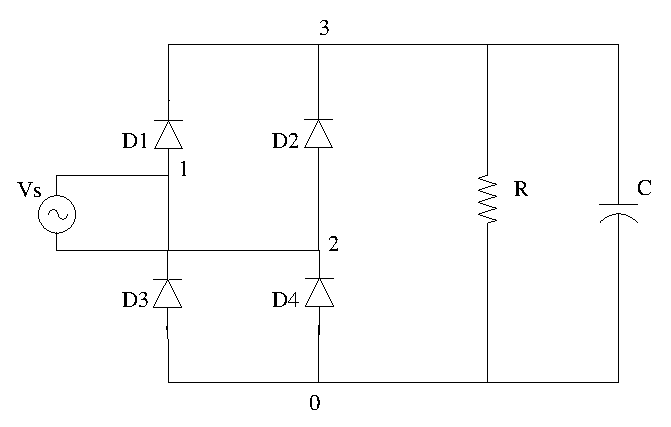
\includegraphics[scale=0.47]{../figures/bridgeFilter.eps}
\end{figure}
\vspace{-0.5cm}
\begin{tiny}
* Full Wave Bridge Rectifier 
\newline
\vspace{-0.1cm}
V1 1 2 sine (5 50) 
\newline
\vspace{-0.1cm}
D1 1 3 mymodel (1e-8 0.026) 
\newline
\vspace{-0.1cm}
D2 2 3 mymodel (1e-8 0.026) 
\newline
\vspace{-0.1cm}
D3 0 1 mymodel (1e-8 0.026) 
\newline
\vspace{-0.1cm}
D4 0 2 mymodel (1e-8 0.026) 
\newline
\vspace{-0.1cm}
R1 3 0 10000 
\newline
\vspace{-0.1cm}
C1 3 0 1e-2 
\newline
\vspace{-0.1cm}
.tran 0 100 0.5 
\newline
\vspace{-0.1cm}
.plot v(1)-v(2) v(3) 
\newline
\vspace{-0.1cm}
.end 
\end{tiny}
\end{minipage}
\hspace{0.1cm} % To get a little bit of space between the figures
\begin{minipage}[!b]{0.47\linewidth} % A minipage that covers half the page
\begin{figure}[h]
\centering
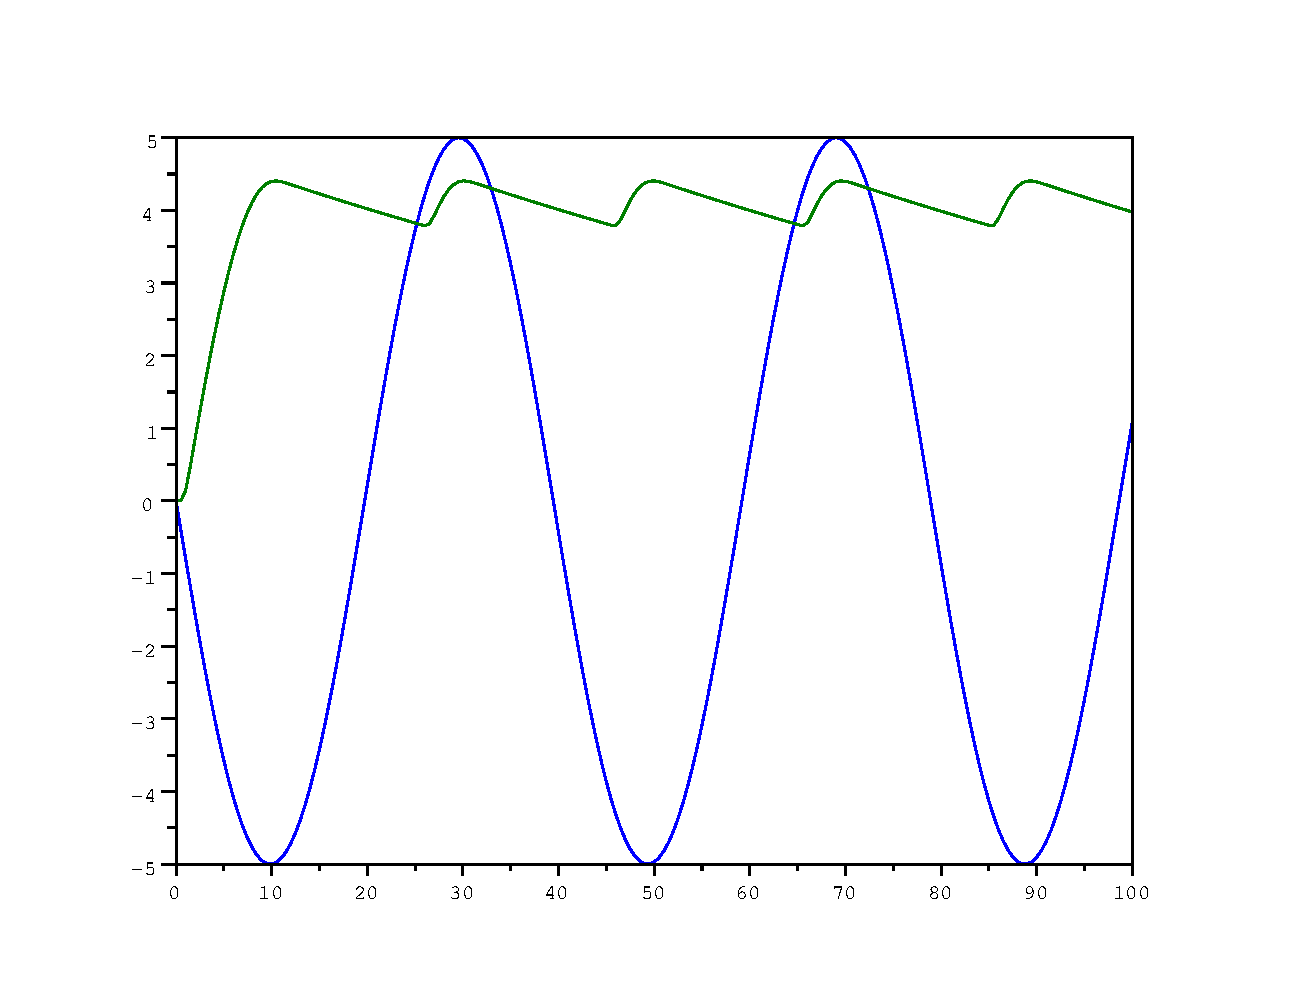
\includegraphics[scale=0.3]{../figures/bridgeFilterOutput.eps}
\caption{Input-Output Waveform} 
\end{figure}
\end{minipage}
\end{frame}

\begin{frame}
 \frametitle{Features}
\begin{itemize}
  \item Various Analysis options.
    \begin{itemize}
      \item Operating Point Analysis
      \item DC Analysis 
      \item Transient Analysis  
      \item AC Analysis 
    \end{itemize}
  \item {\color{red} Facility to define a new component.}
  \item Provides circuit equations for debugging as well as learning circuit simulator.
  \item Easy to integrate and test a new method such as convergence technique, integration method etc. 
\end{itemize} 
\end{frame}

\begin{frame}
\frametitle{User defined Components}
Consider, a non-linear resistance,
$$I=\frac{1}{R}V^3$$

\begin{itemize}
\item Create  a file \$CompName.sci
\item Define
\begin{itemize}
\item Function in the $i=g(v)$ form
\item Jacobian of the function
\end{itemize}
\end{itemize}

%{\bf Syntax:-}
%\newline
%function I=\$CompName\_func(voltage,parameter)
%\$par\_2=parameter(2)
%\$par\_3=parameter(3)
\end{frame}

\begin{frame}
\frametitle{Non-linear Resistance}
\begin{minipage}[!b]{0.43\linewidth} % A minipage that covers half the page
\begin{figure}[h]
\centering
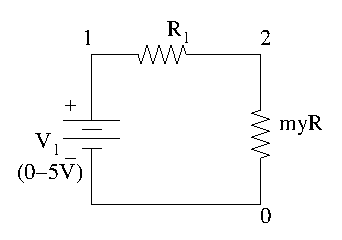
\includegraphics[scale=0.7]{../figures/myR.eps}
\end{figure}
\begin{tiny}
function I=myR\_func(voltage,param)\newline
\hspace*{1cm}R=param(2); \newline
\hspace*{1cm}I=1/R*(voltage$^3$);\newline
endfunction 

function Gj=myR\_Jacobian(voltage,param)\newline 
\hspace*{1cm}R=param(2); \newline
\hspace*{1cm}Gj=3/R*(voltage$^2$);\newline
endfunction
\end{tiny}
\end{minipage}
\hspace{0.5cm} % To get a little bit of space between the figures
\begin{minipage}[!b]{0.5\linewidth} % A minipage that covers half the page
\begin{figure}[h]
\centering
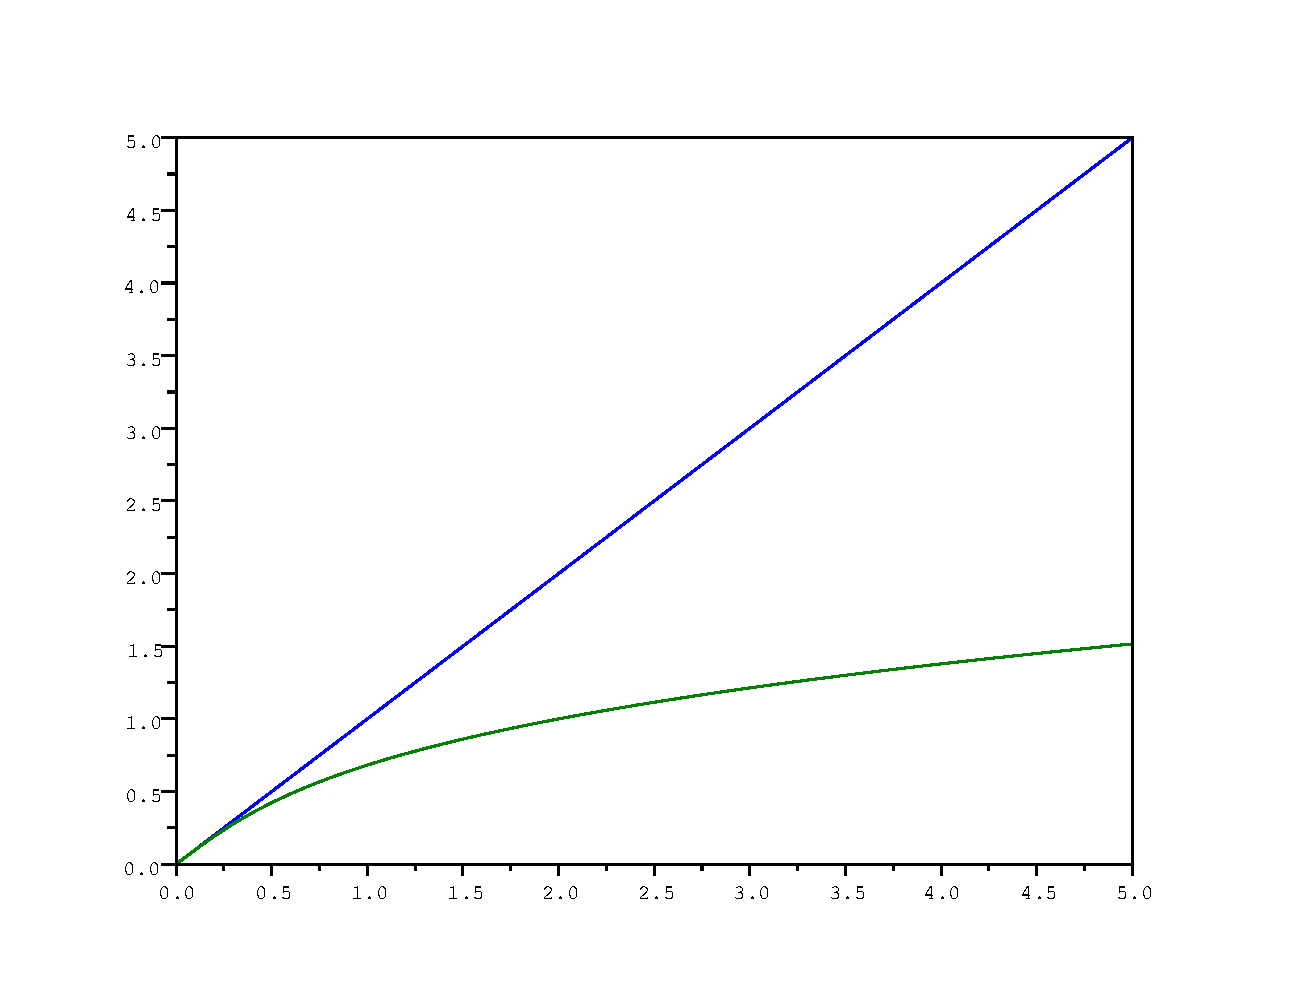
\includegraphics[scale=0.3]{../figures/myROutput.eps}
\end{figure}
\end{minipage}
\end{frame}

\begin{frame}
 \frametitle{Features}
\begin{itemize}
  \item Various Analysis options.
    \begin{itemize}
      \item Operating Point Analysis
      \item DC Analysis 
      \item Transient Analysis  
      \item AC Analysis 
    \end{itemize}
  \item Facility to define a new component.
  \item {\color{red} Provides circuit equations for debugging as well as learning circuit simulator.}
  \item Easy to integrate and test a new method such as convergence technique, integration method etc. 
\end{itemize} 
\end{frame}

\begin{frame}
\begin{block}{Example}
%\begin{minipage}[!b]{0.4\linewidth} % A minipage that covers half the page
\begin{figure}[!ht]
\begin{center}
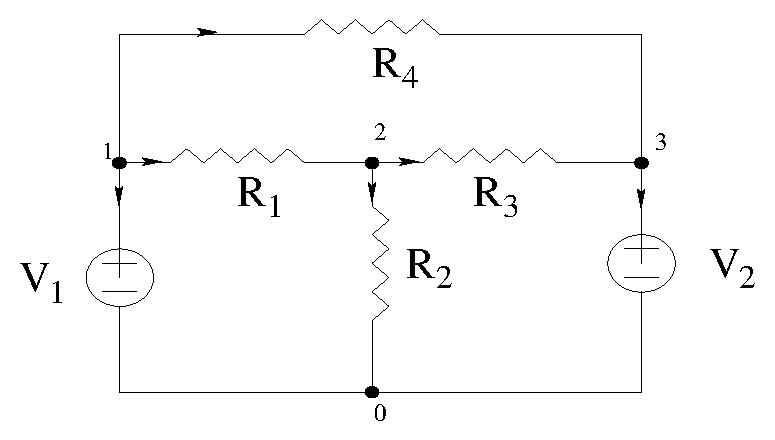
\includegraphics[scale=0.35]{../figures/modified_figure.eps}
\caption{ Example for MNA } \label{modifiedfig}
\end{center}
\end{figure}
%\end{minipage}
%\begin{minipage}[!b]{0.55\linewidth} % A minipage that covers half the page
\begin{tiny}
$$\left[
\begin{array}{cccccc}
G_{1}+G_{4} & -G_{1} & -G_{4} & 1 & 0 \\
-G_{1} & G_{1}+G_{2}+G_{3} & -G_{3} & 0 & 0 \\
-G_{4} & -G_{3} & G_{3}+G_{4} & 0 & 1  \\
1 & 0 & 0 & 0 & 0 \\
0 & 0 & 1 & 0 & 0
\end{array}
\right] \left[
\begin{array}{c}
v_{1}\\
v_{2}\\
v_{3}\\
i_{V_1}\\
i_{V_2}\\
\end{array}
\right]= \left[
\begin{array}{c}
0\\
0\\
0\\
V_{1}\\
V_{2}
\end{array}
\right]$$
\end{tiny}
%\end{minipage}
\end{block}
\end{frame}

\begin{frame}
 \frametitle{Features}
\begin{itemize}
  \item Various Analysis options.
    \begin{itemize}
      \item Operating Point Analysis
      \item DC Analysis 
      \item Transient Analysis  
      \item AC Analysis 
    \end{itemize}
  \item Facility to define a new component.
  \item Provides circuit equations for debugging as well as learning circuit simulator.
  \item {\color{red} Easy to integrate and test a new method such as convergence technique, integration method etc.} 
\end{itemize} 
\end{frame}

\begin{frame}
	\begin{center}
	{\Huge	Thank You}
\end{center}
%	\smiley
\end{frame}
% 
% \section{Operating Point Analysis}
% \begin{frame}
% \begin{block}{Operating Point (OP) Analysis}
% \begin{itemize}
% \item OP Analysis is the central part of a circuit simulator.
% \item The equations that describe the electrical system are nonlinear and algebraic and their solution gives operating point.
% \item Systems of nonlinear equations are solved by iteratively formulating and solving systems of linear algebraic equations. 
% \item The overall efficiency of a circuit simulator is dependent upon the performance of the linear DC analyzer.
% %\item Thus, our work is towards improving the performance of linear DC Analyzers and handling convergence issues related to large size nonlinear circuits.
% \end{itemize}
% \end{block}
% \end{frame}
% 
% \begin{frame}
% \begin{block}{\small Nodal Analysis}
% \begin{itemize}
% \begin{small}
% \item Applicable when the network has only current sources and conductances type devices i.e., $i=g(v)$.
% \item Let, $\mathbf{A}_r$ be the reduced incidence matrix of $\cal{G}$ which is a representative matrix of $V_v(\cal{G})$. \\
% \end{small}
% \begin{tiny}
% The KCL constraints are
% $$\mathbf{A_ri}=\mathbf{0}$$
% $$\left[\begin{array}{cc}
%   \mathbf{A}_{rG} & \mathbf{A}_{rJ}
% \end{array}\right]
% \left[\begin{array}{c}
%   \mathbf{i}_{G} \\
%   \mathbf{i}_{J}
% \end{array}\right]
% =\mathbf{0}$$
% $$\mathbf{A}_{rG}\mathbf{i}_{G}=-\mathbf{A}_{rJ}\mathbf{i}_{J}$$
% 
% $$\mathbf{A}_{rG}\mathbf{G}\mathbf{v}_{G}=-\mathbf{A}_{rJ}\mathbf{i}_{J}\ \ \ \ \ \ \ \ (As, \mathbf{i}_{G}=\mathbf{G}\mathbf{v}_{G})$$
% 
% The KVE constraints are
% $$\left[\begin{array}{c}
%   \mathbf{v}_{G} \\
%   \mathbf{v}_{J}
% \end{array}\right]
% =
% \left[\begin{array}{c}
%   \mathbf{A}_{rG}^T \\
%   \mathbf{A}_{rJ}^T
% \end{array}\right]
% \mathbf{v}_n$$
% 
% \begin{equation}
% \mathbf{A}_{rG}\mathbf{G}\mathbf{A}_{rG}^{T}\mathbf{v}_{n}=-\mathbf{A}_{rJ}\mathbf{i}_{J}
% \label{nodal_equation}
% \end{equation}
% \end{tiny}
% \end{itemize}
% \end{block}
% \end{frame}
% 
% \begin{frame}
% \begin{block}{Matrix Formulation}
% \begin{itemize}
% \item The diagonal entries of the matrix are the sum of conductances incident on the corresponding nodes.
% \item The off diagonal entries $(i,j)^{th}$ of the matrix is the negative of conductances between node $i$ and $j$.
% \item The $\mathbf{A}_{rJ}\mathbf{i}_{J}$ is the sum of current sources leaving the nodes.
% \end{itemize}
% \end{block}
% \begin{block}{Example}
% \end{block}
% \begin{minipage}[!b]{0.4\linewidth} % A minipage that covers half the page
% \begin{figure}[h]
% \centering
% 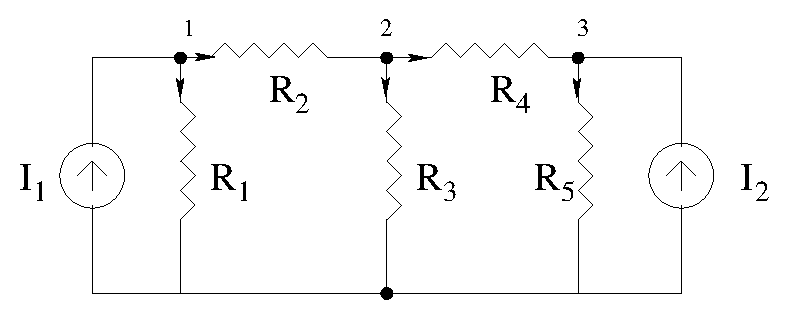
\includegraphics[scale=0.35]{../figures/nodal_figure.eps}
% \end{figure}
% \end{minipage}
% \begin{minipage}[!b]{0.55\linewidth} % A minipage that covers half the page
% \begin{tiny}
% $$\left[
% \begin{array}{ccc}
% G_{1}+G_{2} & -G_{2} & 0\\
% -G_{2} & G_{2}+G_{3}+G_{4} & -G_{4}\\
% 0 & -G_{4} & G_{4}+G_{5}
% \end{array}
% \right] \left[
% \begin{array}{c}
% v_{1}\\
% v_{2}\\
% v_{3}
% \end{array}
% \right]= \left[
% \begin{array}{c}
% I_{1}\\
% 0\\
% I_{2}
% \end{array}
% \right]$$
% \end{tiny}
% \end{minipage}
% \end{frame}
% 
% 
% \begin{frame}
% \begin{block}{Modified Nodal Analysis}
% \begin{small}
% \begin{itemize}
% \item applicable to all kinds of networks.
% \item Let $\mathbf{A}_{r}$ be the reduced incidence matrix of ${\cal{G}}$
% By Tellegan's theorem,
% \begin{tiny}
% $$\mathbf{A_ri}=\mathbf{0}$$
% $$\left[\begin{array}{ccc}
%   \mathbf{A}_{rG} & \mathbf{A}_{rT} & \mathbf{A}_{rJ}
% \end{array}\right]
% \left[\begin{array}{c}
%   \mathbf{i}_{G} \\
%   \mathbf{i}_{T} \\
%   \mathbf{i}_{J}
% \end{array}\right]
% =\mathbf{0}$$
% 
% $$\left[\begin{array}{cc}
%   \mathbf{A}_{rG}\mathbf{G} & \mathbf{A}_{rT}
% \end{array}\right]
% \left[\begin{array}{c}
%   \mathbf{v}_{G} \\
%   \mathbf{i}_{T}
% \end{array}\right]
% =-\mathbf{A}_{rJ}\mathbf{i}_{J}$$
% 
% \begin{equation}
% \label{mna_eq1}
% \left[\begin{array}{cc}
%   \mathbf{A}_{rG}\mathbf{G}\mathbf{A}_{rG}^{T} & \mathbf{A}_{rT}
% \end{array}\right]
% \left[\begin{array}{c}
%   \mathbf{v}_{n} \\
%   \mathbf{i}_{T}
% \end{array}\right]
% =-\mathbf{A}_{rJ}\mathbf{i}_{J}
% \end{equation}
% 
% Device characteristics of the branches in $T$ be
% $$\left[\begin{array}{cc}
%   \mathbf{M} & \mathbf{N}
% \end{array}\right]
% \left[\begin{array}{c}
%   \mathbf{i}_{T} \\
%   \mathbf{v}_{T}
% \end{array}\right]
% =\mathbf{S}_{T}$$
% 
% \begin{equation}
% \label{mna_eq2}
% \left[\begin{array}{cc}
%   \mathbf{NA}_{rT}^{T} & \mathbf{M}
% \end{array}\right]
% \left[\begin{array}{c}
%   \mathbf{v}_{n} \\
%   \mathbf{i}_{T}
% \end{array}\right]
% =\mathbf{S}_{T}
% \end{equation}
% \end{tiny}
% \end{itemize}
% \end{small}
% \end{block}
% \end{frame}
% 
% \begin{frame}
% \begin{block}{Example}
% %\begin{minipage}[!b]{0.4\linewidth} % A minipage that covers half the page
% \begin{figure}[!ht]
% \begin{center}
% 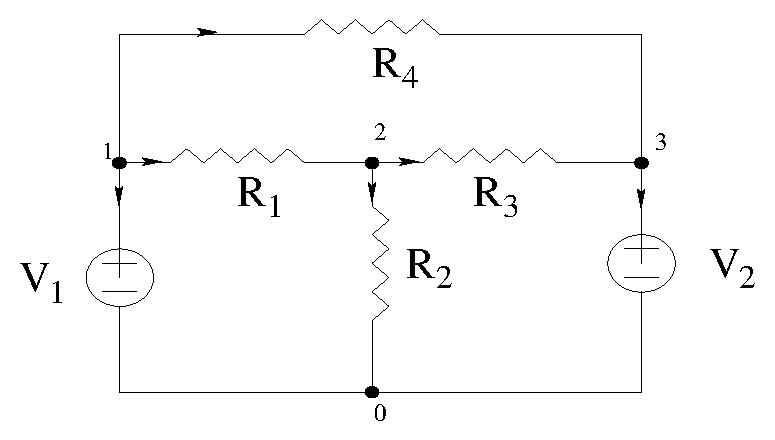
\includegraphics[scale=0.35]{../figures/modified_figure.eps}
% \caption{ Example for MNA } \label{modifiedfig}
% \end{center}
% \end{figure}
% %\end{minipage}
% %\begin{minipage}[!b]{0.55\linewidth} % A minipage that covers half the page
% \begin{tiny}
% $$\left[
% \begin{array}{cccccc}
% G_{1}+G_{4} & -G_{1} & -G_{4} & 1 & 0 \\
% -G_{1} & G_{1}+G_{2}+G_{3} & -G_{3} & 0 & 0 \\
% -G_{4} & -G_{3} & G_{3}+G_{4} & 0 & 1  \\
% 1 & 0 & 0 & 0 & 0 \\
% 0 & 0 & 1 & 0 & 0
% \end{array}
% \right] \left[
% \begin{array}{c}
% v_{1}\\
% v_{2}\\
% v_{3}\\
% i_{V_1}\\
% i_{V_2}\\
% \end{array}
% \right]= \left[
% \begin{array}{c}
% 0\\
% 0\\
% 0\\
% V_{1}\\
% V_{2}
% \end{array}
% \right]$$
% \end{tiny}
% %\end{minipage}
% \end{block}
% \end{frame}
% 
% \begin{frame}
% \frametitle{Controlled Sources}
% \begin{minipage}[!b]{0.47\linewidth} % A minipage that covers half the page
%   \begin{figure}[!ht]
%       \centering
%       
\includegraphics[scale=0.6]{../figures/VCCS.eps}
%       \caption{Voltage Controlled Current Source (VCCS)}
%       \label{vccs}
%   \end{figure}
% \end{minipage}
% %\hspace{0.5cm} % To get a little bit of space between the figures
% \begin{minipage}[!b]{0.47\linewidth}
%   \begin{figure}[!ht]
%      \centering
%       
\includegraphics[scale=0.6]{../figures/VCVS.eps}
%       \caption{Voltage Controlled Voltage Source (VCVS) }
%       \label{vcvs}
%   \end{figure}
%     \end{minipage}
% \begin{minipage}[!b]{0.47\linewidth} % A minipage that covers half the page
%   \begin{figure}[!ht]
%       \centering
%       
\includegraphics[scale=0.6]{../figures/CCCS.eps}
%       \caption{Current Controlled Current Source (CCCS)}
%       \label{cccs}
%   \end{figure}
% \end{minipage}
% %\hspace{0.5cm} % To get a little bit of space between the figures
% \begin{minipage}[!b]{0.47\linewidth}
%   \begin{figure}[!ht]
%      \centering
%       
\includegraphics[scale=0.6]{../figures/CCVS.eps}
%       \caption{Current Controlled Voltage Source (CCVS) }
%       \label{ccvs}
%   \end{figure}
%     \end{minipage}
% \begin{small}
% \begin{itemize}
% \item In voltage controlled devices, we have added a $0A$ current source as controlling branch
% %without disturbing the incidence relationship of existing edges (i.e., the addition is 'soldering type') and its voltage is used for calculating the value of the devices.
% \item In current controlled devices, we have added a $0V$ voltage source as controlling branch
% %by splitting a node (i.e., plier type entry) and the current through it is used for calculating the value of the devices.
% \end{itemize}
% \end{small}
% \end{frame}
% 
% \begin{frame}
% \frametitle{Linearization of Nonlinear Elements}
% \begin{minipage}[!b]{0.5\linewidth}
% Diode characteristics,
% $$I_D=I_S(e^{qV/kT}-1)$$
% $$I_D=I_D|_{V=V_0} + (V-V_0)\frac{I_D}{V}|_{V=V_0}$$
% $$I_D=I_{D0}+(V-V_0)G_{D0}$$
% \begin{figure}[h]
% \begin{center}
% 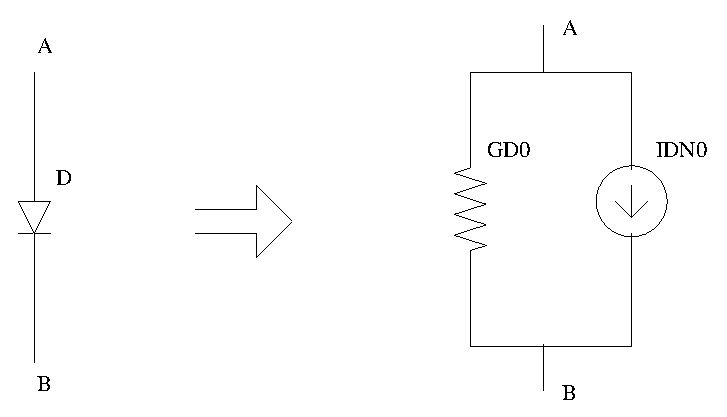
\includegraphics[scale=0.4]{../figures/diodeI.eps}
% \begin{small}Modeling of Diode\end{small}
% \label{diodeI}
% \end{center}
% \end{figure}
% \end{minipage}
% \begin{minipage}[!b]{0.4\linewidth}
% \begin{figure}[h]
% \begin{center}
% 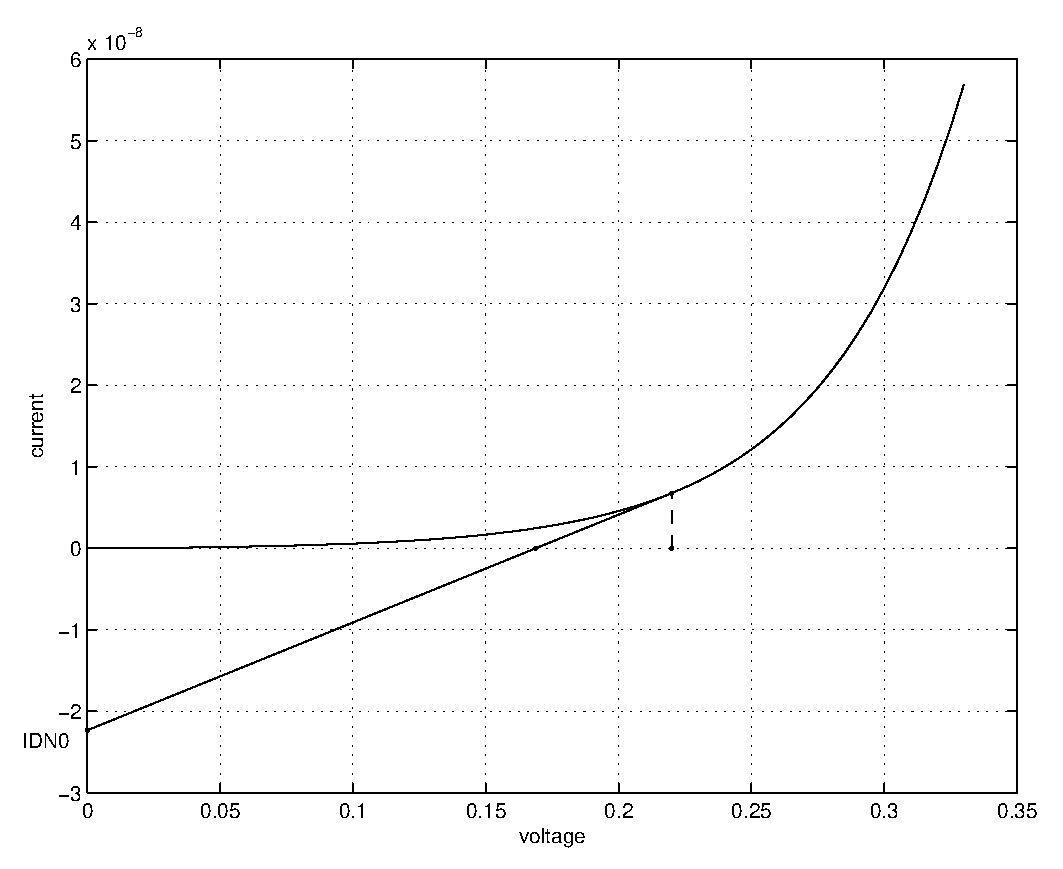
\includegraphics[scale=0.3]{../figures/diodechar1.eps}
% \begin{small}Linearized approximation of diode model\end{small}
% \begin{tiny}$$I_{DN0}=I_{D0}-V_0G_{D0}$$\end{tiny}
% \end{center}
% \end{figure}
% \end{minipage}
% \end{frame}
% 
% 
% \begin{frame}
% {\bf Procedure:}{Operating Point Analysis}
% \small
% \begin{algorithmic}[1]
% \STATE Find Node Potential and Current through devices whose device characteristic can not be expressed in terms of voltage.
% \STATE Find branch voltage and node potentail.
% \STATE Find branch current from branch voltage using device characteristics.
% \IF{Non-linear component}
% \STATE {\bf NR:} Check  device characteristics of non-linear devices.
% \IF {Device characteristics is not satisfied}
% \STATE Call Newton Raphson procedure
% \STATE Find Node Potential and Current through devices whose device characteristic can not be expressed in terms of voltage.
% \STATE Find branch current from branch voltage using device characteristics.
% \STATE Go to {\bf NR}
% \ENDIF
% \STATE Check for KCL
% \ENDIF
% \end{algorithmic}
% \normalsize
% \end{frame}
% 
% \begin{frame}
% \frametitle{Full Wave Bridge Rectifier}
% \begin{minipage}[!b]{0.4\linewidth} % A minipage that covers half the page
% \begin{figure}[h]
% \centering
% 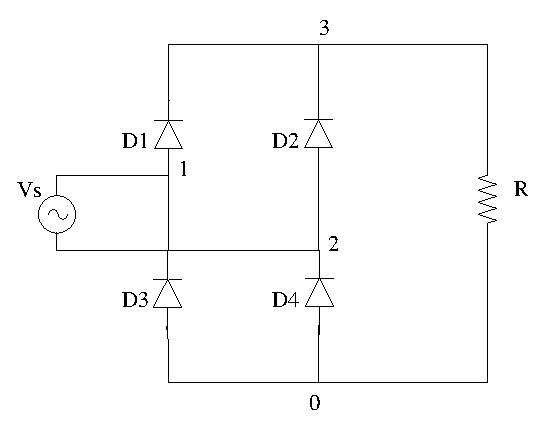
\includegraphics[scale=0.5]{../figures/bridge.eps}
% \end{figure}
% \end{minipage}
% \hspace{0.5cm} % To get a little bit of space between the figures
% \begin{minipage}[!b]{0.5\linewidth} % A minipage that covers half the page
% \begin{figure}[h]
% \centering
% 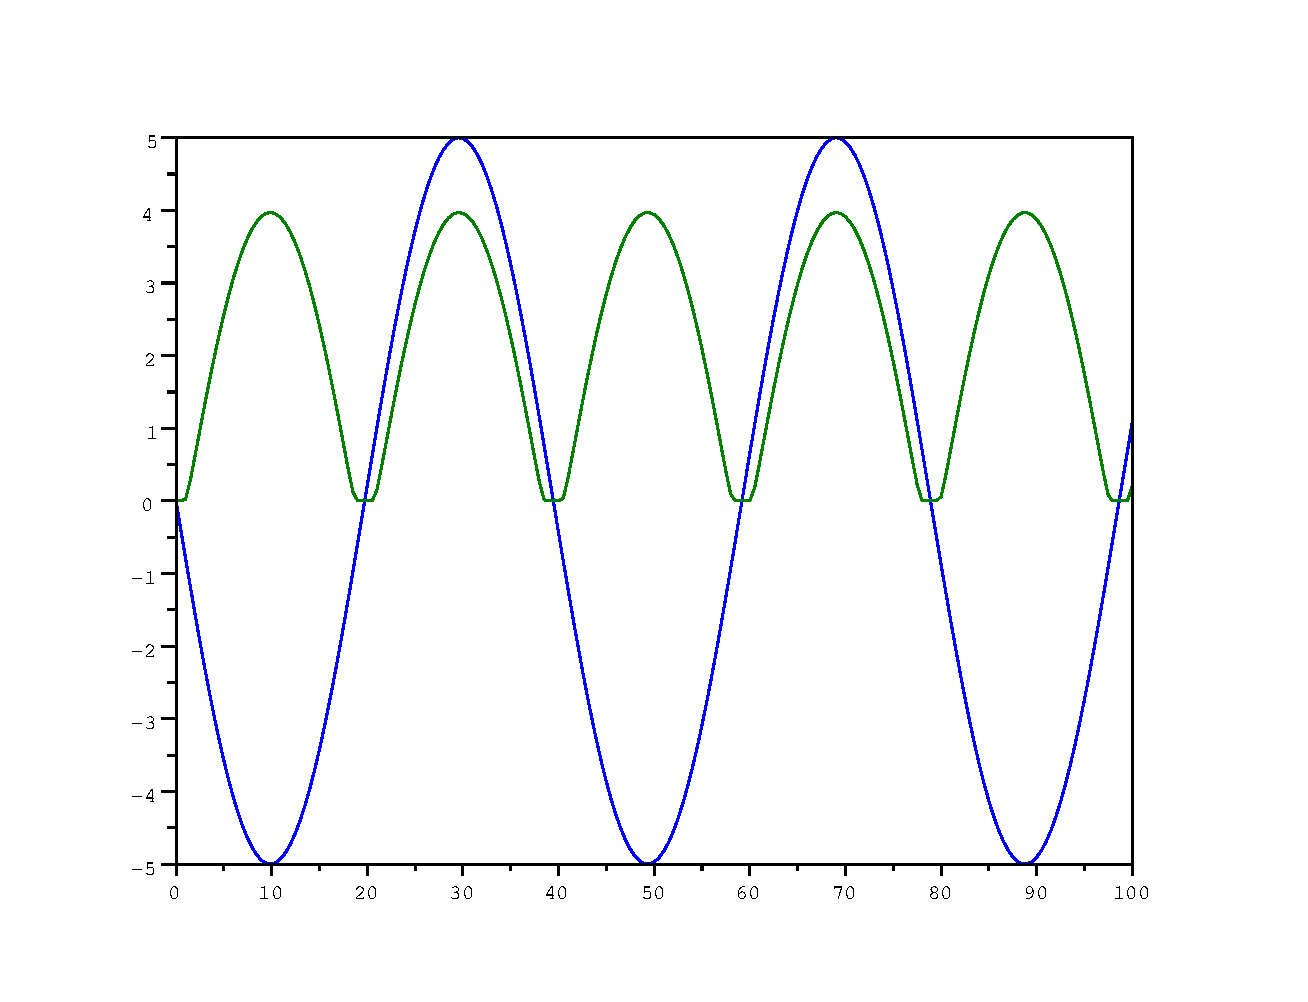
\includegraphics[scale=0.3]{../figures/bridgeOutput.eps}
% \end{figure}
% \end{minipage}
% \end{frame}
% 
% \section{DC Analysis}
% \begin{frame}
% \frametitle{DC Analysis}
% {\bf Procedure:}{DC Analysis}
% \small
% \begin{algorithmic}[1]
% \STATE Modify the value of the sweep source and update Modified Nodal matrix.
% \STATE Do Operating Point Analysis.
% \end{algorithmic}
% \normalsize
% \end{frame}
% 
% \begin{frame}
% \frametitle{Voltage Sweep}
% \begin{minipage}[!b]{0.4\linewidth} % A minipage that covers half the page
% \begin{figure}[h]
% \centering
% 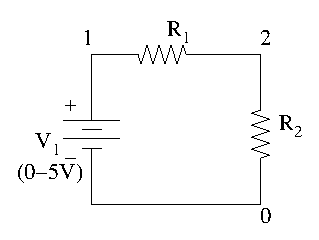
\includegraphics[scale=0.8]{../figures/V_Sweep.eps}
% \caption{Example of DC Analysis (Vsweep.ckt)}
% \end{figure}
% \end{minipage}
% \hspace{0.5cm} % To get a little bit of space between the figures
% \begin{minipage}[!b]{0.5\linewidth} % A minipage that covers half the page
% \begin{figure}[h]
% \centering
% 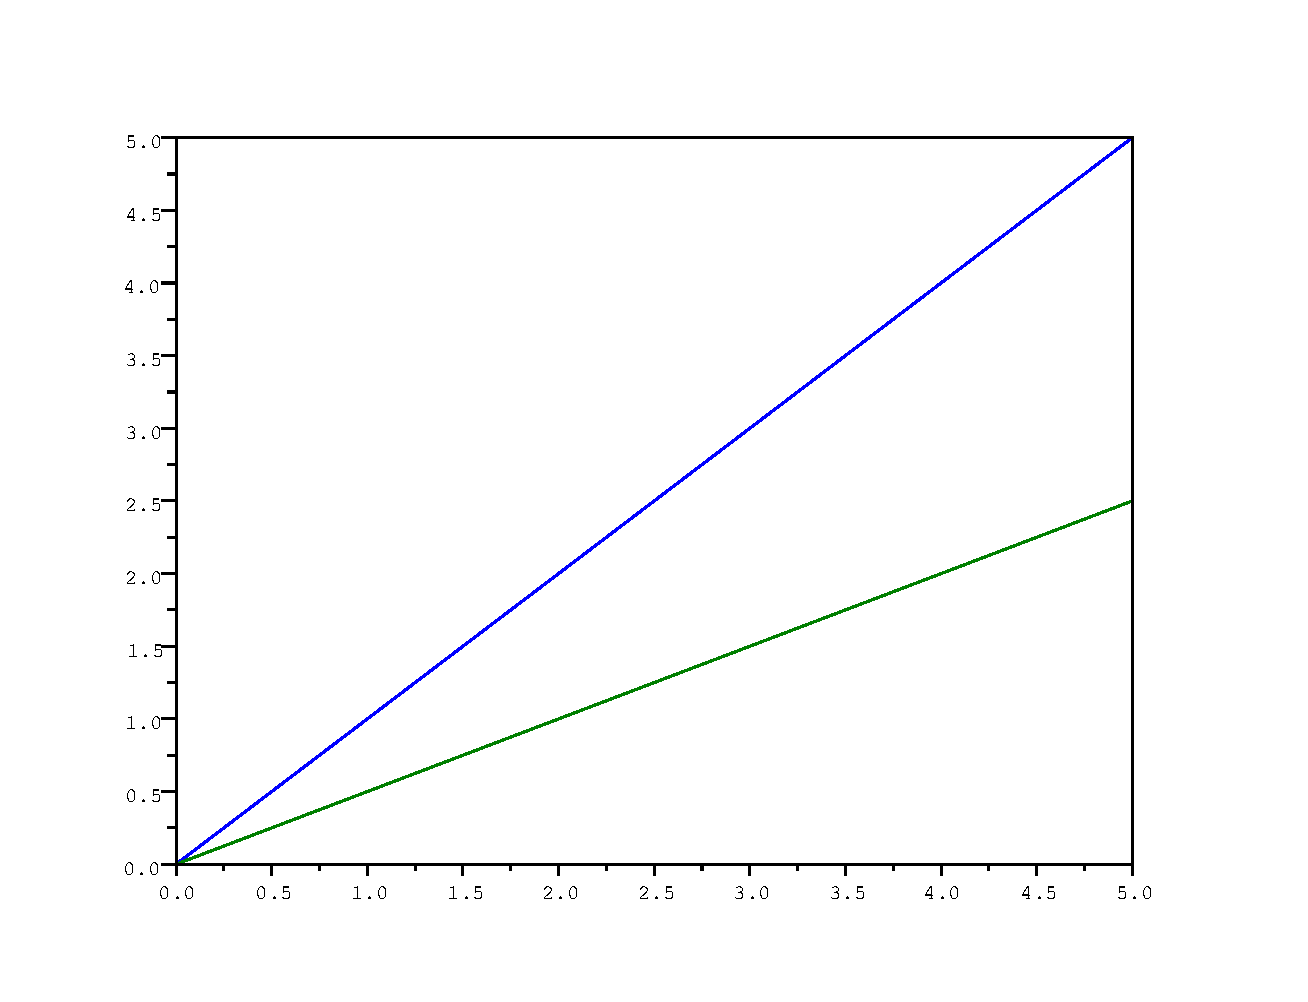
\includegraphics[scale=0.3]{../figures/V_SweepOutput.eps}
% \end{figure}
% \end{minipage}
% \end{frame}
% 
% \section{Transient Analysis}
% \begin{frame}
%   \begin{block}{What is Transient Analysis?}
%      \begin{itemize}
%        \item Computes the response of a circuit as function of time.
%        \item Time is discretized and the solution is computed piecewise.
%      \end{itemize}
%    \end{block}
%   \begin{block}{Important factors}
%     \begin{itemize}
%       \item Proper time Stepping.
%       \item Integration methods.
%     \end{itemize}
%   \end{block}
% \end{frame}
% 
% \begin{frame}
% \frametitle{Discreatization}
% Consider, a capacitor
% \begin{tiny}
% $$I_C(t_n)=C\frac{\partial{V}_C(t_n)}{\partial{t}}$$
% Using Backward Euler's method,
% $$I_C(t_n)=C\frac{V(t_n)-V(t_{n-1})}{t_n-t_{n-1}}$$
% $$I_C(t_n)=\frac{C}{h}V(t_n)-\frac{C}{h}V(t_{n-1})$$
% $$I_C(t_n)=G_C^{(k)}V(t_n)-I_C^{(k)}$$
% \end{tiny}
% \begin{figure}[h]
% \centering
% 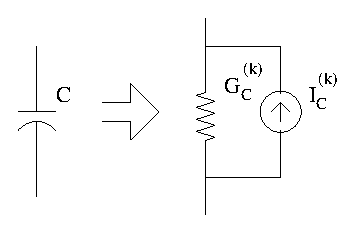
\includegraphics[scale=0.8]{../figures/Ceq.eps}
% \end{figure}
% \end{frame}
% 
% \begin{frame}
% \frametitle{RC Circuit}
% \begin{minipage}[!b]{0.4\linewidth} % A minipage that covers half the page
% \begin{figure}[h]
% \centering
% 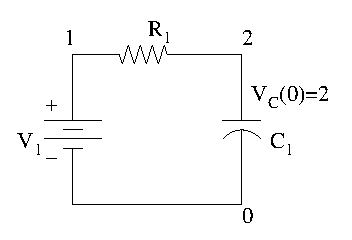
\includegraphics[scale=0.8]{../figures/RC.eps}
% \end{figure}
% \end{minipage}
% \hspace{0.5cm} % To get a little bit of space between the figures
% \begin{minipage}[!b]{0.5\linewidth} % A minipage that covers half the page
% \begin{figure}[h]
% \centering
% 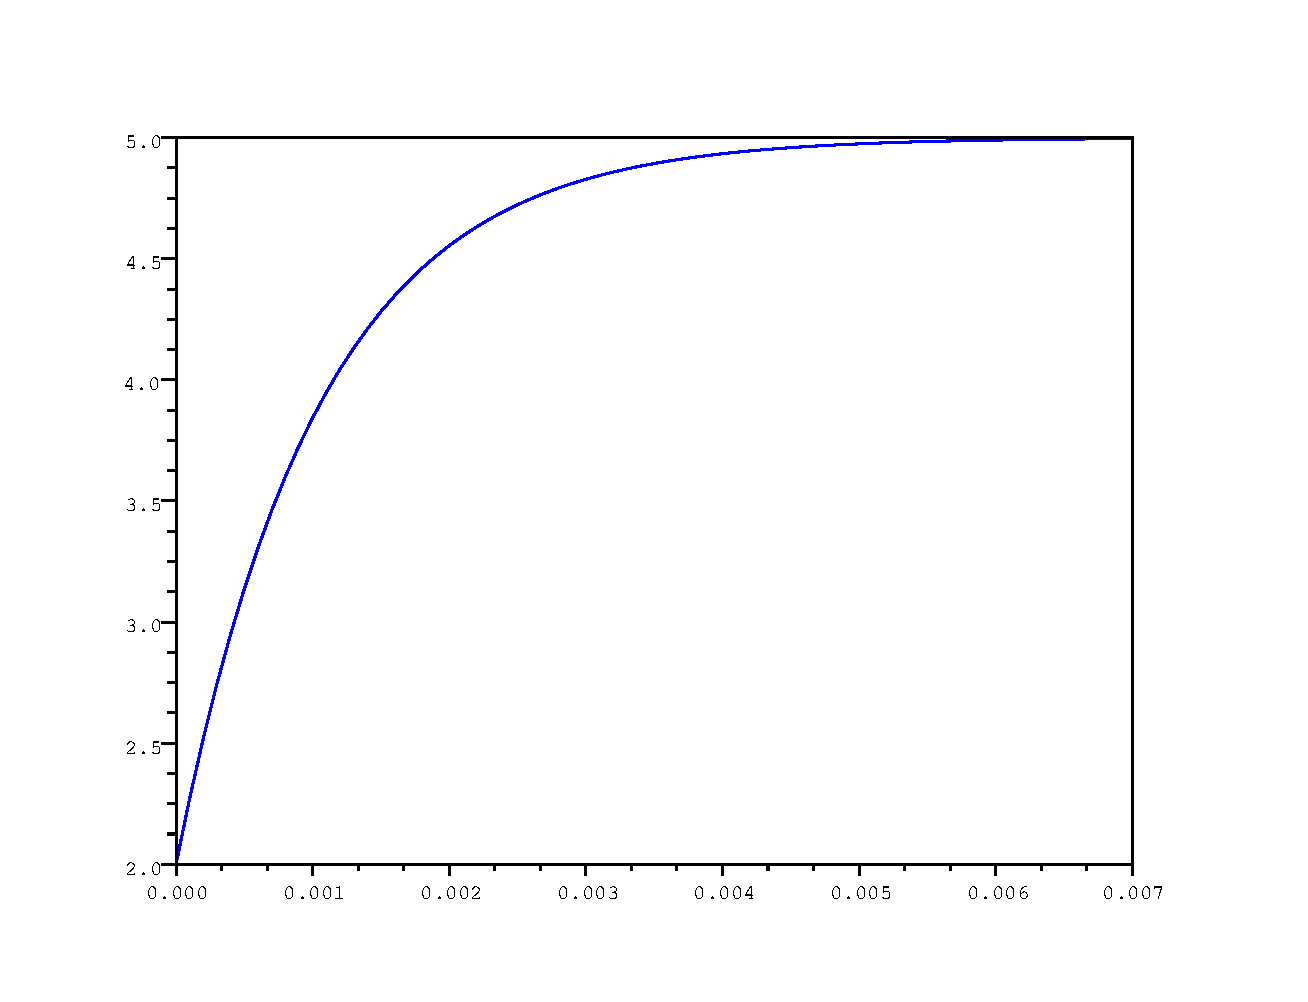
\includegraphics[scale=0.3]{../figures/RCOutput.eps}
% \end{figure}
% \end{minipage}
% \end{frame}
% 
% 
% \begin{frame}
% \frametitle{PseudoCode}
% {\bf Procedure:}{Transient Analysis}
% \small
% \begin{algorithmic}[1]
% \STATE Discretize time dependent Component and Update Modified Nodal matrix.
% \STATE Do Operating Point Analysis.
% \end{algorithmic}
% \normalsize
% 
% {\bf Procedure:}{Discretization}
% \small
% \begin{algorithmic}[1]
% \STATE Compute time dependent source value at time t.
% \STATE Compute the values of static model of dynamic component at time t.
% \STATE Update Modified Nodal matrix.
% \end{algorithmic}
% \normalsize
% \end{frame}
% 
% %\begin{frame}
% %\frametitle{CMOS Inverter}
% %\begin{minipage}[!b]{0.4\linewidth} % A minipage that covers half the page
% %\begin{figure}[h]
% %\centering
% %\includegraphics[scale=0.4]{../figures/inverter.eps}
% %\end{figure}
% %\end{minipage}
% %\hspace{0.5cm} % To get a little bit of space between the figures
% %\begin{minipage}[!b]{0.5\linewidth} % A minipage that covers half the page
% %\begin{figure}[h]
% %\centering
% %\includegraphics[scale=0.3]{../figures/inverterOutput.eps}
% %\end{figure}
% %\end{minipage}
% %\end{frame}
% 
\end{document}

